\chapter{Data Selection}
\label{cha:data_selection}
The selected dataset onto which a classification model shall be learned is provided by Kaggle \footnote{2017 Kaggle Inc}. It is named \textit{The movies Dataset}\footnote{Link to the dataset: \hyperref[https://www.kaggle.com/rounakbanik/the-movies-dataset]{https://www.kaggle.com/rounakbanik/the-movies-dataset}} and contains metadata on approximately 45,000 movies in its raw format. It is provided and updated by Rounik Banik. The csv-file has 24 columns.\\\\
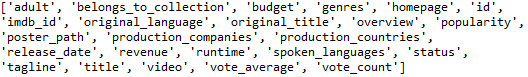
\includegraphics[width=\textwidth]{images/Raw_dataset_headers.png}
Untertitel bla bla


\textcolor{red}{\textit{unvollstaendige daten erlaeutern, grundlegende Graphen zeichnen lassen}}




\begin{itemize}
	\item In slides named: "structure and size of data"
	\item min. 1 Page
	\item Selection: 
	\begin{itemize}
		\item What data is available?
		\item What do I know about the provenance of the data?
		\item What do I know about the quality of the data?
	\end{itemize}
	\item Exploration
	\begin{itemize}
		\item Get an initial understanding of the data
		\item Calculate basic summarization statistics
		\item Visualize the data
		\item Identify data problems such as outliers, missing values, duplicate records
	\end{itemize}
\end{itemize}

